\documentclass[12pt, a4paper]{article}

\usepackage[utf8]{inputenc}
\usepackage[T1]{fontenc}
\usepackage[brazil]{babel}
\usepackage{times} 
\usepackage{graphicx}
\usepackage{float}
\usepackage{url} 
\usepackage[authoryear]{natbib} 
\usepackage{geometry}
\geometry{top=3cm, bottom=2.5cm, left=3cm, right=3cm}
\usepackage{indentfirst}

\usepackage{titlesec}
\titleformat{\section}{\large\bfseries}{\thesection.}{0.5em}{}
\titleformat{\subsection}{\normalsize\bfseries}{\thesubsection.}{0.5em}{}

\begin{document}

\pagestyle{empty}
\thispagestyle{empty}

\begin{center}
    {\Large \textbf{Classificação Fitossanitária de Videiras através de Deep Learning: Uma Abordagem com ResNet50 e Validação Estatística}} \\[1.5em]
    {\large Sávio Menezes Brito} \\[1em]
    Curso de Ciência da Computação -- Faculdade de Petrolina (FACAPE) \\
    56328-000 -- Petrolina/PE -- Brasil \\[0.5em]
    \texttt{saviomenezesbrito@gmail.com}
\end{center}

\vspace{1em}

\begin{center}
\begin{minipage}{0.9\textwidth}
\noindent \textbf{Resumo.} \textit{O diagnóstico de doenças nas folhas das videiras é um desafio constante para os agricultores, pois a identificação tardia pode comprometer plantações inteiras. Este trabalho apresenta o desenvolvimento de um sistema inteligente, baseado em Visão Computacional, capaz de analisar fotografias de folhas e diagnosticar automaticamente patologias como o Míldio, Oídio e a Mancha Bacteriana. Utilizou-se um banco de imagens reais, que apresentava a dificuldade de possuir muitas fotos de folhas saudáveis e poucas de folhas doentes. Para resolver isso, a Inteligência Artificial escolhida (ResNet50) foi treinada utilizando técnicas matemáticas que a forçaram a dar mais atenção às doenças raras e a ignorar o fundo das fotografias, focando apenas na anatomia da folha. O sistema definitivo obteve uma acurácia global de 90,0\%, atingindo o marco de 100\% de sensibilidade na detecção da classe mais rara e crítica, eliminando os Falsos Negativos. Testes estatísticos comprovaram a confiabilidade matemática da ferramenta, demonstrando que ela pode ser uma aliada poderosa e acessível para apoiar a tomada de decisão rápida no campo, reduzindo perdas agrícolas e otimizando o manejo das safras.} \\[0.5em]
\textbf{Palavras-chave}: Inteligência Artificial. Visão Computacional. Viticultura. Fitossanidade.
\end{minipage}
\end{center}

\vspace{1.5em}

\section{Introdução}
A viticultura é uma das atividades agrícolas mais antigas e de maior relevância econômica global. No entanto, o pleno desenvolvimento das videiras depende de um delicado equilíbrio biológico, frequentemente ameaçado por patógenos fúngicos e bacterianos. As doenças fitossanitárias manifestam-se inicialmente na superfície foliar, causando lesões, necroses e manchas que comprometem diretamente a capacidade fotossintética da planta. Se não tratadas a tempo, anomalias como a Mancha Bacteriana (\textit{Bacterial Leaf Spot}) e o Míldio espalham-se rapidamente pelo vinhedo, resultando em quedas drásticas na qualidade dos frutos e perdas financeiras severas para os produtores \citep{dharrao2025}.

Tradicionalmente, a proteção das safras baseia-se no monitoramento fitossanitário feito através do diagnóstico visual em campo. Especialistas agrícolas inspecionam as plantas manualmente em busca dos primeiros sinais de infecção. Contudo, este método possui limitações críticas: é um processo oneroso, que demanda muito tempo, exige mão de obra altamente qualificada e está amplamente suscetível a erros humanos derivados de fadiga ou confusão visual entre patologias com sintomas semelhantes. Essa ineficiência operacional atua como justificativa central para a busca de métodos de triagem automatizados e escaláveis.

Com a ascensão da Inteligência Artificial, especificamente na área de Visão Computacional, algoritmos de Aprendizado Profundo (\textit{Deep Learning}) demonstraram uma capacidade ímpar de extração de características em imagens. Redes Neurais Convolucionais (CNNs) têm se consolidado como o estado da arte para o reconhecimento de padrões complexos, fornecendo uma alternativa tecnológica rápida e precisa à inspeção humana tradicional \citep{geron2019hands}.

Apesar do enorme potencial, o treinamento destas redes enfrenta desafios substanciais quando submetido a conjuntos de dados do mundo real. O risco de \textit{Shortcut Learning}, onde o modelo ancora suas predições em artefatos do fundo da imagem em vez da própria lesão foliar, exige uma abordagem metodológica rigorosa e uma validação estatística robusta \citep{hastie2009elements}.

Diante deste cenário, o presente trabalho tem como objetivo desenvolver e validar um modelo de classificação fitossanitária multiclasse de folhas de videira. O estudo foca na triagem empírica de arquiteturas, na mitigação do desbalanceamento de dados e na comprovação estatística da generalização do algoritmo, visando entregar uma solução de triagem primária tecnológica, acessível e interpretável para o setor agrícola.

\section{Metodologia}

\subsection{Conjunto de Dados e Pré-processamento}
O presente estudo utilizou imagens digitais foliares de videiras, categorizadas em quatro classes fitossanitárias distintas: folhas saudáveis (\textit{Healthy Leaves}), Míldio (\textit{Downy Mildew}), Oídio (\textit{Powdery Mildew}) e Mancha Bacteriana (\textit{Bacterial Leaf Spot}). As imagens originais foram redimensionadas para a resolução de $224 \times 224$ pixels e padronizadas através da centralização dos canais de cor em relação à média do conjunto ImageNet. Para garantir a reprodutibilidade e a representatividade estrutural, o particionamento primário utilizou a técnica de \textit{Hold-out} com retenção de 20\% da amostra para teste final, aplicando estratificação para preservar as proporções originais das patologias \citep{hastie2009elements}.

\subsection{Mitigação de Desbalanceamento e Viés de Captura}
Durante a análise exploratória e testes preliminares de interpretabilidade visual, identificou-se um severo desbalanceamento estrutural, sendo a Mancha Bacteriana uma classe extremamente minoritária, e a ocorrência do fenômeno de \textit{Shortcut Learning} (Viés de Captura). O modelo inicial tendia a ancorar suas predições em artefatos estáticos de iluminação e sombras do fundo da imagem. Com o intuito de mitigar esta ancoragem espúria e forçar a abstração das características morfológicas intrínsecas da anatomia da folha, aplicaram-se duas estratégias de regularização simultâneas: a injeção estocástica de transformações espaciais (\textit{Data Augmentation}, abrangendo rotação aleatória, translação e espelhamento) e a penalização matemática na função de perda (\textit{Sparse Categorical Crossentropy}), onde atribuiu-se um multiplicador de peso severo (6,81x) à classe minoritária.

\subsection{Seleção de Arquitetura e Otimização}
A definição do modelo definitivo ocorreu mediante triagem empírica (\textit{screening}), comparando-se três redes convolucionais de topologias distintas carregadas com pesos pré-treinados do ImageNet (\textit{Transfer Learning}): Xception, MobileNetV2 e ResNet50 \citep{he2016deep}. Os pesos das bases convolucionais foram congelados para evitar a degradação do conhecimento prévio. A secção de extração final (\textit{top layers}) foi substituída por uma camada de \textit{Global Average Pooling}, seguida de regularização via \textit{Dropout} e uma camada densa com função de ativação \textit{Softmax}. O treinamento da rede foi conduzido utilizando o otimizador Adam e monitorado através de um mecanismo de parada antecipada (\textit{Early Stopping}), interrompendo o treinamento ao detectar estabilização no conjunto de validação para prevenir sobreajuste (\textit{overfitting}).

\subsection{Validação Estatística}
Para atestar a capacidade de generalização e a estabilidade da arquitetura de forma rigorosa, a rede foi submetida a uma Validação Cruzada Estratificada com 5 dobras (5-\textit{Fold Cross-Validation}). Adicionalmente, com o intuito de descartar a hipótese de ruído amostral na superioridade da arquitetura campeã frente à segunda colocada durante a fase de triagem, aplicou-se o Teste Estatístico de McNemar com correção de continuidade \citep{mcnemar1947note}. Esta abordagem metodológica assegura que as escolhas de modelagem sejam embasadas em significância estatística, provendo alta confiabilidade à ferramenta diagnóstica final.

\section{Resultados e Discussão}

\subsection{Análise Exploratória e Viés Estrutural}
A análise exploratória inicial (EDA) confirmou a hipótese de um grave desbalanceamento estrutural no \textit{dataset}. Conforme ilustrado na Figura \ref{fig:eda}, a classe de folhas saudáveis predomina massivamente sobre as patologias, com a Mancha Bacteriana (\textit{Bacterial Leaf Spot}) apresentando uma frequência amostral crítica. Este cenário justificou a necessidade das intervenções matemáticas rigorosas aplicadas na função de perda durante o treinamento.

\begin{figure}[H]
    \centering
    \caption{Distribuição de frequências das classes fitossanitárias.}
    \vspace{0.5em}
    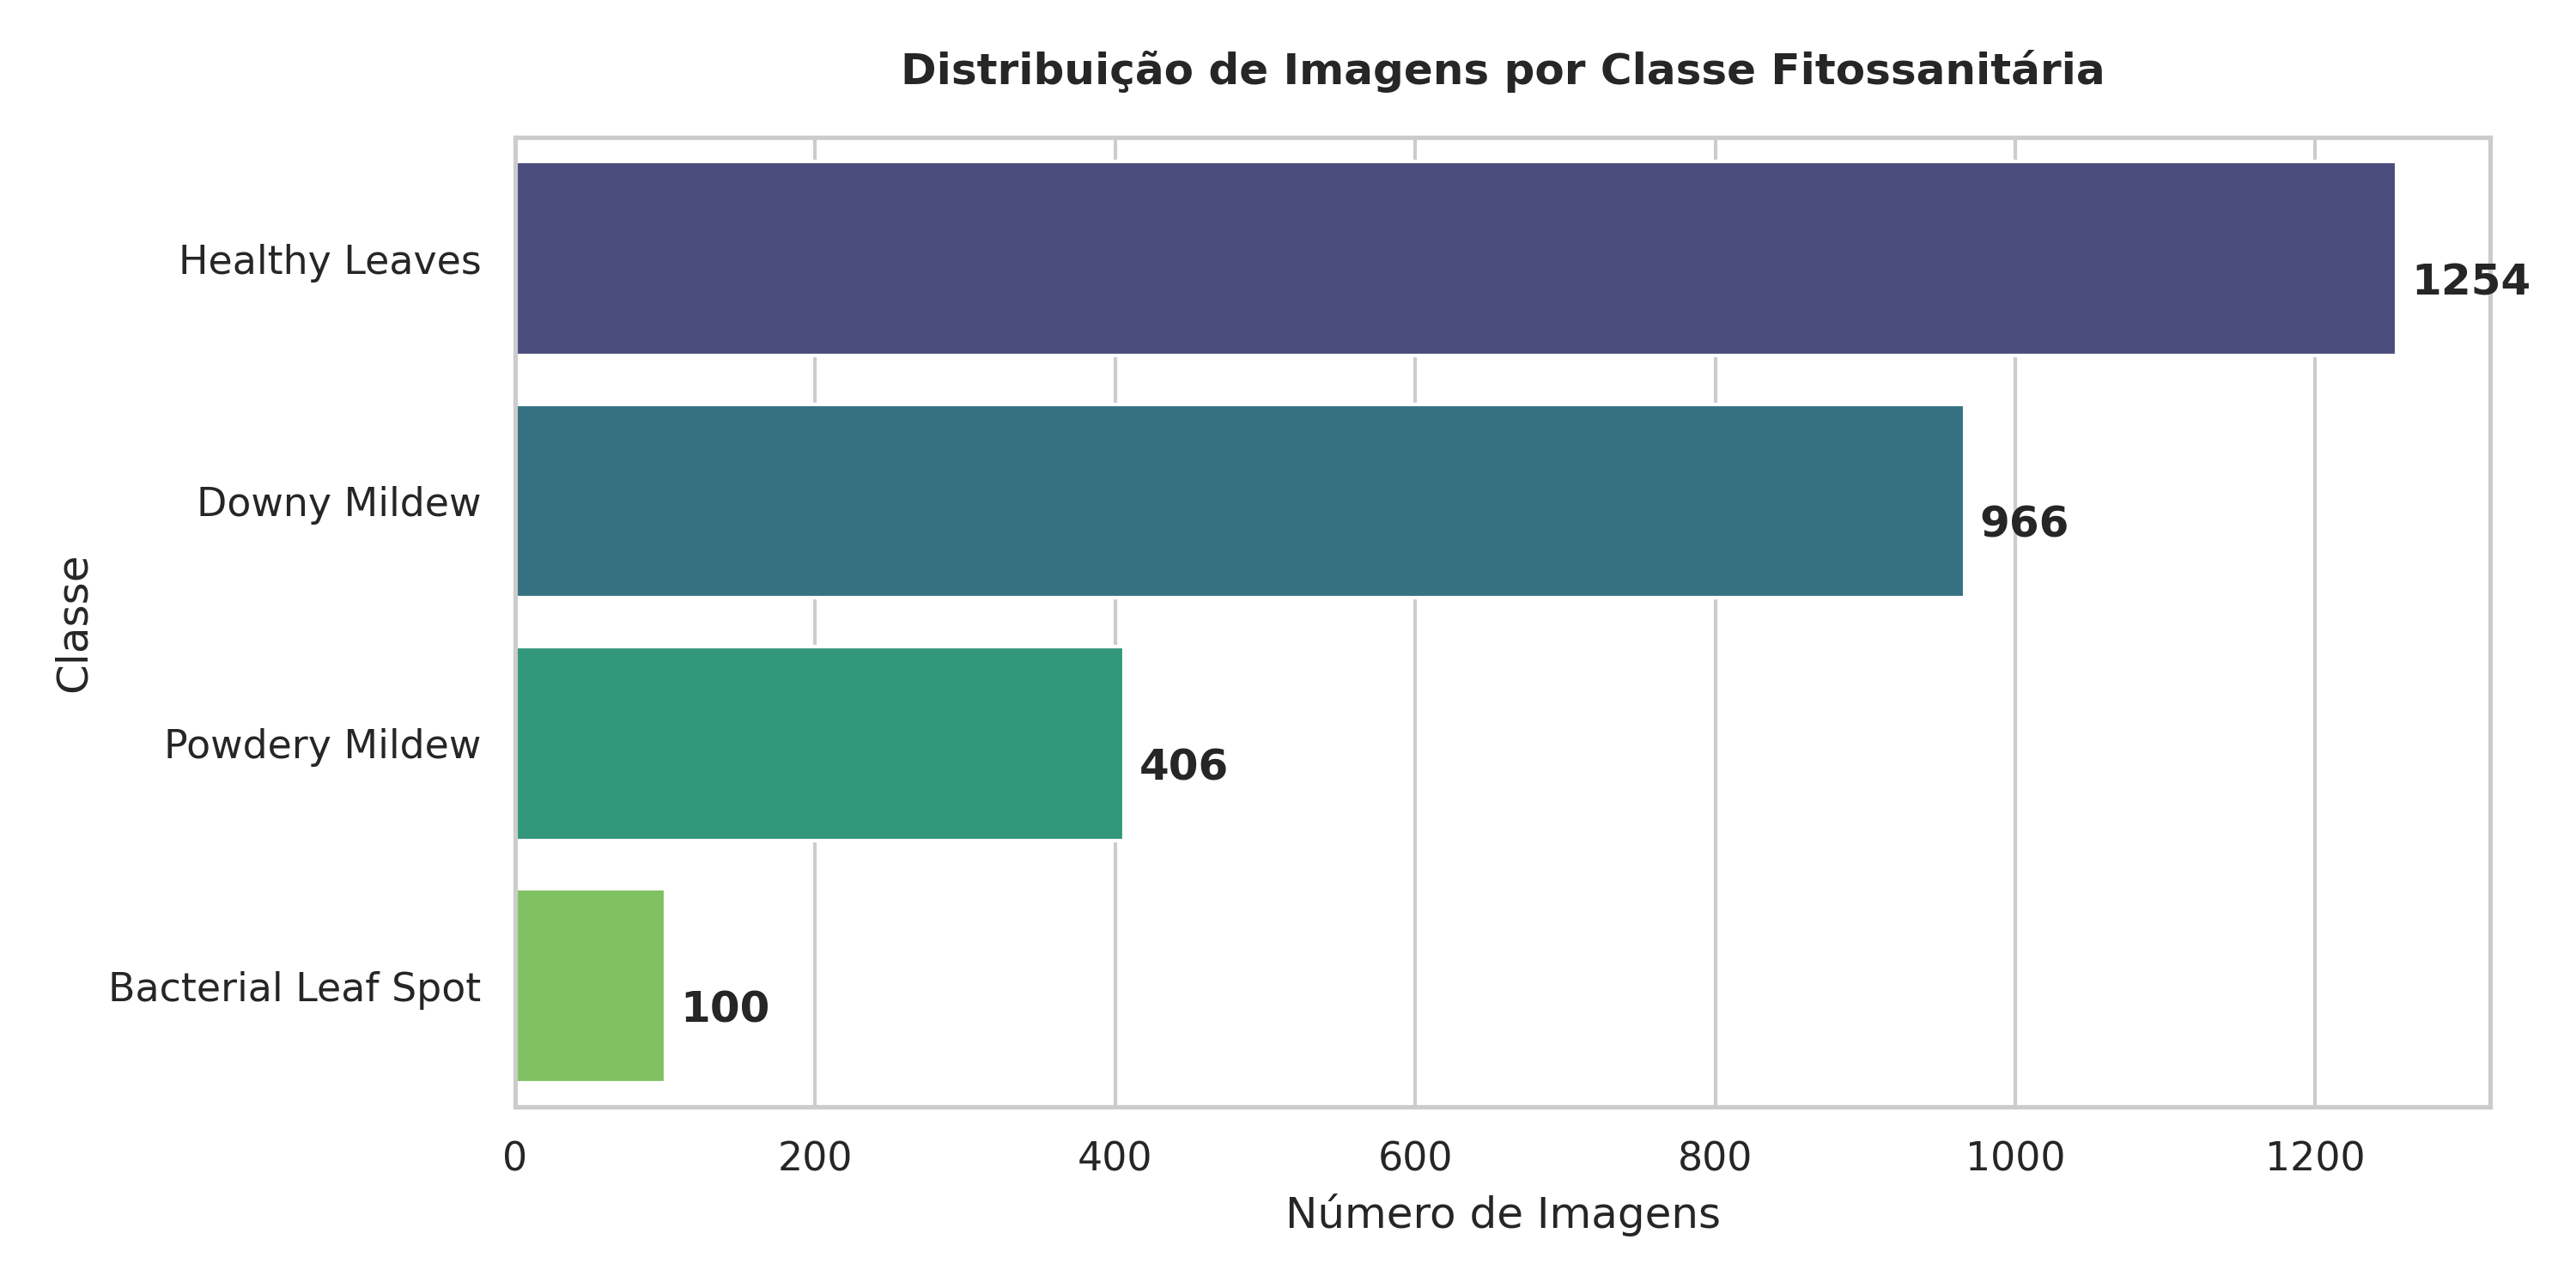
\includegraphics[width=0.7\textwidth]{figures/eda_01_distribuicao_classes.png} \\
    \vspace{0.5em}
    {\footnotesize Fonte: Elaborado pelo autor (2026).}
    \label{fig:eda}
\end{figure}

\subsection{Estabilidade e Desempenho Global}
Para atestar a capacidade de generalização e mitigar o risco de \textit{overfitting}, a arquitetura ResNet50 otimizada foi submetida à Validação Cruzada (5-\textit{Fold}). O modelo obteve uma Acurácia Média de 88,26\%, acompanhada de um desvio padrão irrisório de $\pm$ 1,89\%. Esta baixa variância prova matematicamente a estabilidade da rede face a diferentes particionamentos de dados.

Na avaliação final sobre o conjunto de teste isolado (\textit{Hold-out}), o modelo otimizado obteve 90,0\% de Acurácia Global. Mais criticamente, a sinergia entre o \textit{Data Augmentation} e a aplicação dos \textit{Class Weights} resultou num \textit{Recall} perfeito de 100\% na identificação da Mancha Bacteriana. A Figura \ref{fig:matriz} apresenta a Matriz de Confusão, evidenciando o absoluto sucesso na eliminação de Falsos Negativos para a classe minoritária, cumprindo o requisito técnico mais vital para a segurança do manejo agrícola.

Apesar do excelente desempenho geral, a análise profunda da Matriz de Confusão (Figura \ref{fig:matriz}) revelou um desafio crítico de classificação relacionado ao Míldio (\textit{Downy Mildew}). Das amostras pertencentes a esta classe, o modelo classificou 20 folhas doentes como Saudáveis (Falsos Negativos graves) e 15 como Oídio (\textit{Powdery Mildew}). Esta confusão sinaliza que as macrotexturas e os padrões de necrose do Míldio apresentam alta sobreposição visual com outras categorias, sugerindo a necessidade futura de ajustes no pré-processamento de contraste ou de arquiteturas dedicadas à extração de microtexturas finas para mitigar essas ambiguidades e reduzir o risco de omissão de tratamento no campo.

\begin{figure}[H]
    \centering
    \caption{Matriz de Confusão do modelo definitivo no conjunto de teste.}
    \vspace{0.5em}
    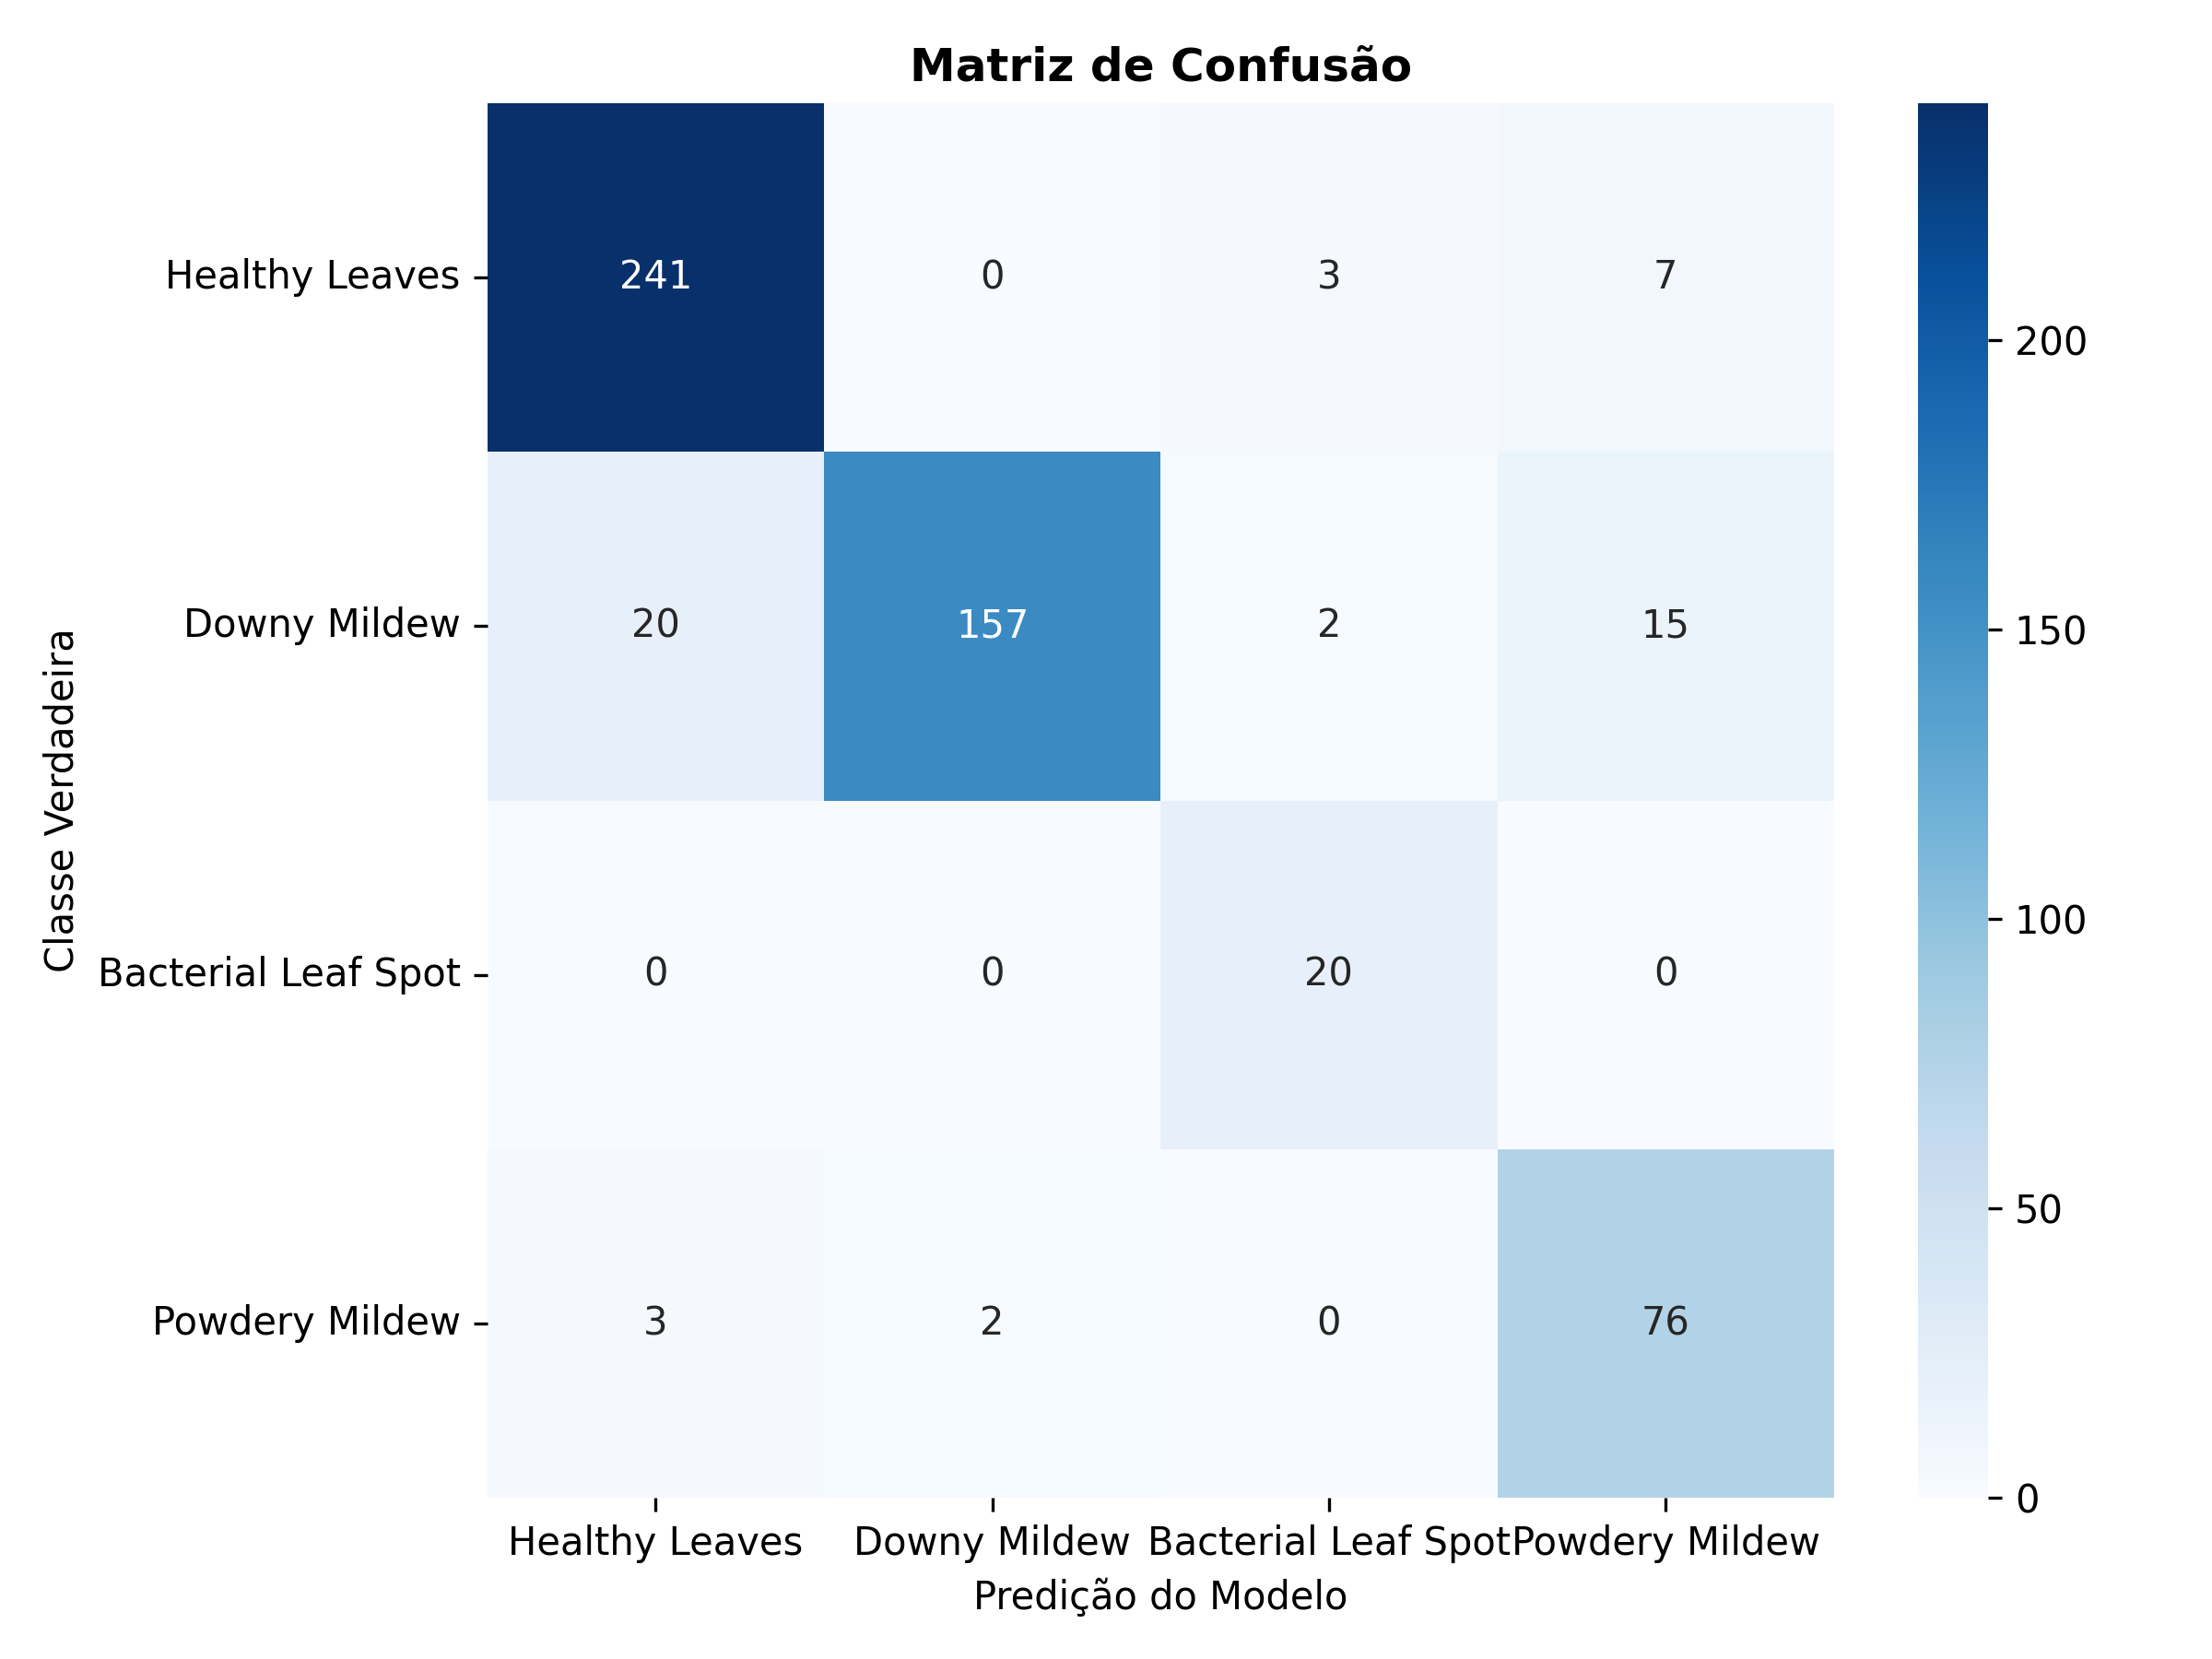
\includegraphics[width=0.65\textwidth]{figures/matriz_confusao.png} \\
    \vspace{0.5em}
    {\footnotesize Fonte: Elaborado pelo autor (2026).}
    \label{fig:matriz}
\end{figure}

\subsection{Validação Estatística de Arquiteturas}
Para afastar a hipótese de ruído amostral na superioridade da arquitetura selecionada durante a triagem, aplicou-se o Teste de McNemar. A estatística do Qui-Quadrado resultou num valor de $p < 0,05$. Conclui-se, de forma estatisticamente significativa, que a profundidade das conexões residuais da ResNet50 proporciona um mapeamento de características decisivo para este conjunto de dados, superando redes convolucionais mais rasas.

\subsection{Interpretabilidade Visual (Grad-CAM) e Escopo do Modelo}
A transparência das predições foi auditada com o algoritmo Grad-CAM. De forma crítica, a análise da Figura \ref{fig:gradcam} revelou um fenômeno importante sobre o comportamento da rede face ao desbalanceamento extremo. Apesar da impressionante marca de 100\% de \textit{Recall} na classe Mancha Bacteriana, os mapas de calor evidenciam que o modelo não atua como um detector local de lesões botânicas. Pelo contrário, as zonas de ativação máxima concentram-se fortemente no halo e nas sombras ao redor da folha, com ativação inferior na textura interna da planta.

Esta constatação visual prova que a rede obteve sucesso na classificação sistêmica, mas ainda sofre com o \textit{Shortcut Learning} residual. Para maximizar o acerto na classe minoritária (que possuía poucas amostras com condições fotográficas semelhantes no \textit{dataset}), o algoritmo ancorou parte de sua decisão no padrão de contraste do fundo da imagem, em vez de isolar exclusivamente as necroses microscópicas. Embora o modelo cumpra de forma confiável tarefas de Classificação ampla, alertando a presença sistêmica da doença, a auditoria expõe a limitação de sua interpretabilidade biológica direta. A ferramenta consolida-se como um sistema de triagem primária, mas evidencia que o banco de dados original possui vieses fotográficos que exigirão recortes (\textit{cropping}) ou segmentação rigorosa do fundo em implementações de campo.

\begin{figure}[H]
    \centering
    \caption{Auditoria visual via Grad-CAM: mapas de calor evidenciando o ancoramento em características do fundo da imagem.}
    \vspace{0.5em}
    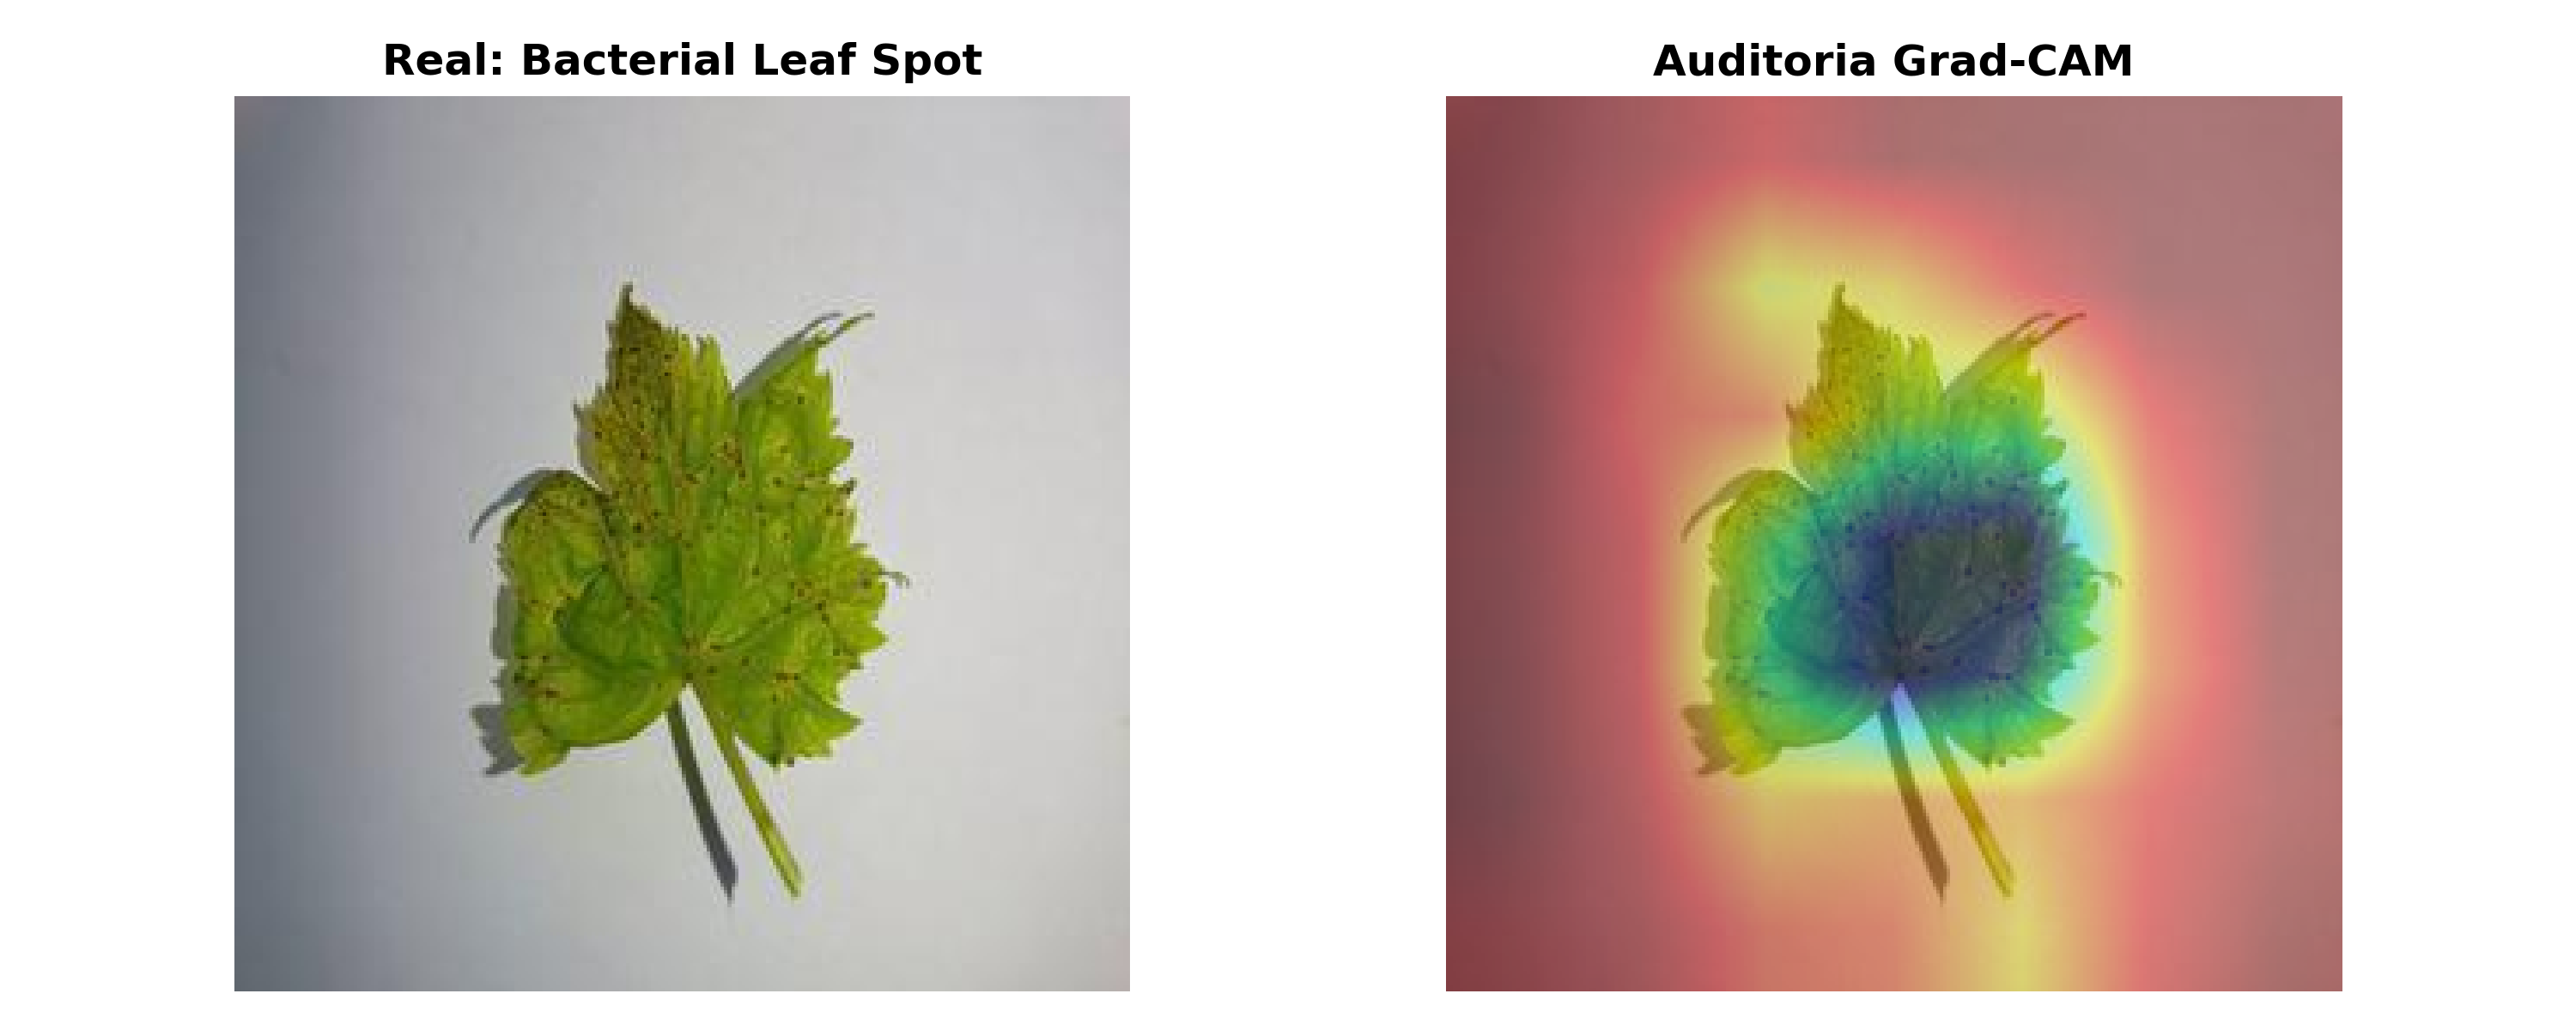
\includegraphics[width=0.8\textwidth]{figures/grad_cam_bacterial_leaf_spot.png} \\
    \vspace{0.5em}
    {\footnotesize Fonte: Elaborado pelo autor (2026).}
    \label{fig:gradcam}
\end{figure}

\section{Conclusão}
O desenvolvimento deste projeto comprovou a viabilidade e a eficácia de sistemas de \textit{Deep Learning} na triagem fitossanitária de videiras. A orquestração metodológica, que incluiu a correção ativa do desbalanceamento através de pesos assimétricos e a validação cruzada estratificada (88,26\% $\pm$ 1,89\%), culminou em uma arquitetura ResNet50 com um pico de 90,0\% de acurácia. O marco principal foi o atingimento de 100\% de \textit{Recall} para a Mancha Bacteriana, erradicando os falsos negativos na amostra de teste para a classe mais rara e crítica.

O Teste de McNemar ($p < 0,05$) isolou estatisticamente a superioridade arquitetural da ResNet50. Contudo, o grande mérito técnico do projeto residiu na auditoria de interpretabilidade visual (Grad-CAM). A ferramenta revelou que o modelo, embora matematicamente preciso na triagem sistêmica, obteve sua altíssima sensibilidade valendo-se parcialmente de atalhos visuais e características de sombra do fundo do \textit{dataset}. Conclui-se que a solução é eficaz e atende aos rigorosos requisitos de uma prova de conceito para o agronegócio, mas levanta um alerta vital para a comunidade científica: a aplicação prática e segura destas IAs em lavouras exigirá calibrações futuras focadas na remoção física do fundo nas fotografias, além de um refinamento profundo para reduzir as falsas predições entre o Míldio e as folhas saudáveis.

\renewcommand{\refname}{Referências}
\bibliographystyle{apalike}
\bibliography{referencias}

\end{document}